\section{ARMA Models}\label{sec:ARMA}
Classical regression is often insufficient for explaining all of the interesting dynamics
of a time series.
Instead, the introduction of correlation that may be generated through lagged linear relations
leads to proposing the \textbf{autoregressive (AR)} and \textbf{autoregressive moving average (ARMA)} models
that were presented in Whittle (1951) \cite{Whittle1951}.


\subsection{White Noise}\label{sec:whitenoise}

In many respects the simplest kind of time series $\{X_t\}$ is one in which
the random variables $X_t,t=0,\pm1,\pm2,\ldots$ are independently and identically distributed with zero mean and variance $\sigma^2.$
From a second order point of view i.e. ignoring all properties of the joint distributions of $\{X_t\}$
except those which can be deduced from the moments $\mathbb{E}[X_t]$ and $\mathbb{E}[X_s X_t]$,
such processes are identified with the class of all stationary processes having mean zero and \textit{autocovariance function}:
\begin{gather}\label{eq:WN}
    \gamma(h)=\Cov[X_t, X_{t+h}]=\begin{cases}
                                \sigma^2 & \mathrm{~if~}h=0,\\
                                0 & \mathrm{~if~}h\neq 0.
                            \end{cases}
\end{gather}

\begin{definition}[White Noise]\label{def:whitenoise}
    \
    
    The process $u_t$ is called \textbf{white noise}, written as
    \begin{gather*}
        u_t \sim WN(\mu, \sigma^2) 
    \end{gather*}
    if and only if $u_t$ has a mean of $\mu$ and covariance function \ref{eq:WN}.
    We call $u_t$ strong WN if $u_t \perp u_{t-h}, \forall t,h$ (i.e. $u_t$ and $u_{t-h}$ are independent).
\end{definition}

Usually, we deal with mean-zero WN: $u_t \sim WN(0, \sigma^2).$
\begin{note}
    \

    The distinction between (weak) WN and strong WN is only important for models where higher moments of $u_t$ matter, e.g.
    conditional heteroskedasticity models.
\end{note}
By this definition \ref{def:whitenoise}, we can easily know that any mean-zero i.i.d. sequence with finite variances (MDS) is a
white noise series. The converse is not true: there exist white noise series' that are not strictly stationary (MDS).

\textit{Therefore, the following types of shocks are nested: i.i.d., MDS, and white noise,
with i.i.d. being the most narrow class and white noise the broadest.}

If the WN process $u_t$ is Normal, then it is strong WN, as linear independence implies independence for Normal RVs.
We can simply write $u_t \overset{i.i.d.}{\sim} \mathcal{N}(0, \sigma^2)$.
Note that the Normal WN process is SS and ergodic as it consists of i.i.d. RVs at each $t$.

\begin{theorem}[Wold Decomposition]\label{thm:wolddecomp}
    \

    Suppose that $\{y_t\}$ is \textit{weak stationary}, with a finite variance (\textit{we shall assume that it has mean zero, though this is not necessary}).
    Then $y_t$ can be uniquely expressed as
    \begin{gather*}
        y_t = \sum_{j=0}^{\infty} \phi_j u_{t-j} + V_t 
    \end{gather*}
    where
    \begin{enumerate}
        \item $\{u_t\} \sim WN(0, \sigma^2)$;
        \item $\phi_0 = 1$ and $\sum_{j=0}^{\infty} \phi_j^2 < \infty$;
        \item $\mathbb{E}[u_t V_s] = 0$ for all $t,s$;
        \item $V_t$ is deterministic.
    \end{enumerate}
\end{theorem}   

The Wold decomposition shows that $y_t$ can be written as a linear function of the white noise projection errors (\textbf{a linear process} that consists of (infinitely many) WN components) plus a deterministic process.
The Wold decomposition is a foundational result for linear time series analysis.
Since any covariance stationary process can be written in this format this justifies linear models as approximations.

The square summability condition $\sum_{j=0}^{\infty} \phi_j^2 < \infty$ ensures that the coefficients approach zero sufficiently quickly so that the impact of any $u_{t-j}$ on $y_t$ diminishes as $j$ increases.
We refer to $u_t$ as the innovation to the process $y_t$ at time $t$.

Note that the Wold decomposition does not restrict the distributional
family of $u_t$, nor does it exclude higher-order dependencies among $u_t$.

If $u_t$ is i.i.d, then $y_t$ is strictly stationary and ergodic as shown by our previous discussion of constituting ergodic process with definition \ref{def:ergodicity-plain}.

\subsection{ARMA\texorpdfstring{$(p,q)$}{(p,q)} Models}\label{sec:ARMApq}

A very wide class of stationary processes can be generated by using white
noise as the forcing terms in a set of linear difference equations. This leads to
the notion of an autoregressive-moving average (ARMA) process.

\begin{definition}[ARMA$(p,q)$ Process]\label{def:ARMApq}
    \
    
    The process $\{ y_t, t=0, \pm1, \pm2, \cdots\}$ is said to be an ARMA$(p,q)$ process if $y_t$ is stationary and for every $t$,
    \begin{gather}\label{eq:ARMApq}
        y_t - \phi_1 y_{t-1} - \cdots - \phi_p y_{t-p} = \alpha + \theta_1 u_{t-1} + \cdots + \theta_q u_{t-q} + u_t
    \end{gather}
    where $u_t \sim WN(0,\sigma^2)$, $\alpha = \mu \left( 1-\phi_1 - \cdots - \phi_p \right)$, $\mathbb{E}[y_t] = \mu$, and $\phi_p, \theta_q \neq 0.$
\end{definition}
The equation \ref{eq:ARMApq} can be written symbolically in the more compact form:
\begin{gather*}
    \phi (B) y_t = \alpha + \theta(B) u_t, t = 0, \pm1, \pm2, \cdots
\end{gather*}
where $\phi $ and $\theta$ are $p^{th}$ and $q^{th}$ order polynomials in the \textbf{backshift operator} $B$:
\begin{gather*}
    \phi (B) = 1 - \phi_1 B - \cdots - \phi_p B^p,\\
    \theta (B) = 1 + \theta_1 B + \cdots + \theta_q B^q
\end{gather*}
where $B$ is defined by:
\begin{gather*}
    B^j y_t = y_{t-j}, \quad j = 0, \pm1, \pm2, \cdots.
\end{gather*}
The polynomials $\phi(B)$ and $\theta(B)$ will be referred to as the \textbf{autoregressive} and \textbf{moving average} polynomials, respectively.

\subsection{Autoregressive Models (AR\texorpdfstring{$(p)$}{(p)})}\label{sec:AR}

Autoregressive models are based on the idea that the current value of the series,
$y_t$, can be explained as a function of $p$ past values: $y_{t-1}, \cdots, y_{t-p},$
where $p$ determines the number of steps into the past needed to forecast the current value.

If $\theta(B) \equiv 1$ in ARMA$(p,q)$ \ref{eq:ARMApq}, then we have the \textbf{autoregressive} model of order $p$ (AR$(p)$):
\begin{definition}[AR$(p)$ Process]\label{def:ARp}
    \
    
    The process $\{ y_t, t=0, \pm1, \pm2, \cdots\}$ is said to be an AR$(p)$ process if $y_t$ is stationary and for every $t$,
    \begin{gather}\label{eq:ARp}
        y_t - \phi_1 y_{t-1} - \cdots - \phi_p y_{t-p} = \alpha + u_t
    \end{gather}
    where $u_t \sim WN(0,\sigma^2)$, $\alpha = \mu \left( 1-\phi_1 - \cdots - \phi_p \right)$, $\mathbb{E}[y_t] = \mu$, $\phi_p \neq 0.$
    This can be written symbolically in the more compact form:
    \begin{gather*}
        \phi (B) y_t = \alpha + u_t, t = 0, \pm1, \pm2, \cdots
    \end{gather*}
    where $\phi (B) = 1 - \phi_1 B - \cdots - \phi_p B^p$.
\end{definition}

\begin{eg}[AR(1) Process]\label{eg:AR1}
    \

    We initiate the investigation of AR models by considering the first-order model, AR(1), given by
    \begin{gather}\label{eq:AR1}
        y_t = \alpha + \phi_1 y_{t-1} + u_t, \quad u_t \sim WN(0, \sigma^2).
    \end{gather}
    Iterating backwards $k$ times, we get:
    \begin{align*}
        y_t &= \alpha + \phi y_{t-1} + u_t = \alpha + \phi \left( \alpha + \phi y_{t-2} + u_{t-1} \right) + u_t\\
        &= \alpha + \phi \alpha + \phi^2 y_{t-2} + \phi u_{t-1} + u_t\\
        &= \cdots \\
        &= \alpha \left( 1 + \phi + \phi^2 + \cdots + \phi^{k-1} \right) + \phi^k y_{t-k} + \sum_{j=0}^{k-1} \phi^j u_{t-j} \\
        &= \frac{\alpha}{1-\phi} + \phi^k y_{t-k} + \sum_{j=0}^{k-1} \phi^j u_{t-j}.
    \end{align*}
    This method suggests that, by continuing to iterate backward, and provided that $\vert \phi \vert < 1$,
    and $\mathbb{V}[y_t] < \infty$, we can represent an AR(1) model as a linear process given by
    \begin{gather}\label{eq:ARstationarysol}
        y_t = \frac{\alpha}{1-\phi} + \sum_{j=0}^{\infty} \phi^j u_{t-j}.
    \end{gather}
    Representation \ref{eq:ARstationarysol} is called the stationary solution of the model.
    In fact, by simple substitution,
    \begin{gather*}
        \underset{y_t}{\underbrace{\sum_{j=0}^{\infty} \phi^j u_{t-j}}} = \frac{\alpha}{1-\phi} +  \phi \underset{y_{t-1}}{\underbrace{\left(\sum_{k=0}^{\infty} \phi^k u_{t-k-1}\right)}} + u_t
    \end{gather*}
    The AR(1) process defined by \ref{eq:ARstationarysol} is stationary with mean
    \begin{gather*}
        \mathbb{E}[y_t] = \mathbb{E}\left[\frac{\alpha}{1-\phi}\right] + \sum_{j=0}^{\infty} \phi^j \mathbb{E}[u_{t-j}] = \frac{\alpha}{1-\phi}
    \end{gather*}
    and autocovariance function,
    \begin{align*}
        \gamma(h) &= \Cov[y_{t+h}, y_t] = \mathbb{E}\left[ \left( \sum_{j=0}^{\infty} \phi^j u_{t+h-j} \right) \left( \sum_{k=0}^{h} \phi^k u_{t-k} \right) \right] \\
        &= \mathbb{E}\left[ \left(u_{t+h} + \cdots + \phi^h u_t + \phi^{h+1} u_{t-1} + \cdots \right) \left( u_t + \phi u_{t-1} + \cdots \right) \right]\\
        &= \sigma^2 \sum_{j=0}^{\infty} \phi^{h+j} \phi^j \\
        &= \sigma^2 \phi^h \sum_{j=0}^{\infty} \phi^{2j} \\
        &= \frac{\sigma^2 \phi^h}{1-\phi^2}, \quad h \geq 0.
    \end{align*}
    Recall that $\gamma(h) = \gamma(-h)$, so we will only exhibit the autocovariance function for $h \geq 0.$
    We know it that the ACF of an AR(1) process is given by
    \begin{gather*}
        \rho(h) = \frac{\gamma(h)}{\gamma(0)} = \phi^h, \quad h \geq 0.
    \end{gather*}
    and $\rho(h)$ satisfies the recursion:
    \begin{gather*}
        \rho(h) = \phi \rho(h-1), \quad h \geq 1.
    \end{gather*}
\end{eg}

So, under $\vert \phi \vert < 1$, the AR(1) process is stable, since the effect of $u_{t-h}$ on $y_t$ dies out as $h \to \infty.$
If instead $\vert \phi \vert > 1$,then this effect diverges to infinity and we have an exploding process.
If $\phi = 1$, provided that $\alpha = 0$, $y_t$ is simply the sum of past innovations $u_t$:
$y_t = \sum_{h=0}^{\infty} u_{t-h}$. In that case, we call yt a unit-root or random walk process (with drift if $\alpha \neq 0$).
Under $\vert \phi \vert \geq 1$, the process is non-stationary and the ACF diverges to infinity.

\textcolor{red}{Extra material Needed}

\begin{eg}[AR(2) Process]\label{eg:AR2}
    \
    
    The AR(2) process is given by
    \begin{gather}\label{eq:AR2}
        y_t = \alpha + \phi_1 y_{t-1} + \phi_2 y_{t-2} + u_t, \quad u_t \sim WN(0, \sigma^2).
    \end{gather}
    This process can also be written as
    \begin{gather*}
        \phi(L) y_t = \alpha + u_t
    \end{gather*}
    where $\phi(L) = 1 - \phi_1 L - \phi_2 L^2$.
    Let $\frac{1}{\alpha_1}$ and $\frac{1}{\alpha_2}$ be the roots of $\phi(L) = 0$,
    we can rewrite the AR(2) model as:
    \begin{gather*}
        \alpha + u_t = (1-\alpha_1 L)(1-\alpha_2 L) y_t
    \end{gather*}
    We would like to find the conditions for the stationarity of $y_t$.
    It turns out that it's convenient to transform the AR(2) model \ref{eq:AR2} into a VAR(1) process.
    Set $\tilde{y}_t = (y_t, y_{t-1})^{\prime}$, which is stationary if and only if $y_t$ is stationary.
    Then equation \ref{eq:AR2} implies that:
    \begin{gather*}
        \begin{bmatrix}
            y_t \\
            y_{t-1}
        \end{bmatrix} = \begin{bmatrix}
            \alpha \\
            0
        \end{bmatrix} + \begin{bmatrix}
            \phi_1 & \phi_2 \\
            1 & 0
        \end{bmatrix} \begin{bmatrix}
            y_{t-1} \\
            y_{t-2}
        \end{bmatrix} + \begin{bmatrix}
            u_t \\
            0
        \end{bmatrix}
    \end{gather*}
    or, in matrix form:
    \begin{gather*}
        \tilde{y}_t = \mathbf{A} \tilde{y}_{t-1} + \tilde{u}_t
    \end{gather*}
    where $\mathbf{A} = \begin{bmatrix}
        \phi_1 & \phi_2 \\
        1 & 0
    \end{bmatrix}$ and $\tilde{u}_t = \begin{bmatrix}
        \alpha + u_t \\
        0
    \end{bmatrix}$.
    The VAR(1) process is strictly stationary and ergodic if the innovations satisfy $\mathbb{E}[\tilde{u}_t] < \infty$ and all the eigenvalues $\lambda$ of $\mathbf{A}$ are less than 1 in absolute value.
    The eigenvalues of $\mathbf{A}$ are the roots of the characteristic polynomial:
    \begin{gather*}
        \lambda^2 - \phi_1 \lambda - \phi_2 = \lambda^2 \phi\left(\frac{1}{\lambda}\right) = 0
    \end{gather*}
    and $\phi(z) = 1 - \phi_1 z - \phi_2 z^2$ is the autoregressive polynomial of the AR(2) model.
    By factoring this polynomial as $\phi (z) = (1 - \lambda_1 z)(1 - \lambda_2 z)$, we can find the roots $\lambda_1$ and $\lambda_2$.
    The quadratic formula shows that these equal
    \begin{gather}\label{eq:lambdadef}
        \lambda_j = \frac{\phi_1 \pm \sqrt{\phi_1^2 + 4\phi_2}}{2}.
    \end{gather}
    These eigenvalues are real if $\phi_1^2 + 4\phi_2 \geq 0$ and are complex conjugates otherwise.
    The AR(2) process is stationary if the solutions $\vert \lambda_j \vert < 1$ for $j = 1, 2$.
    % \begin{figure}[ht!]
    %     \centering
    %     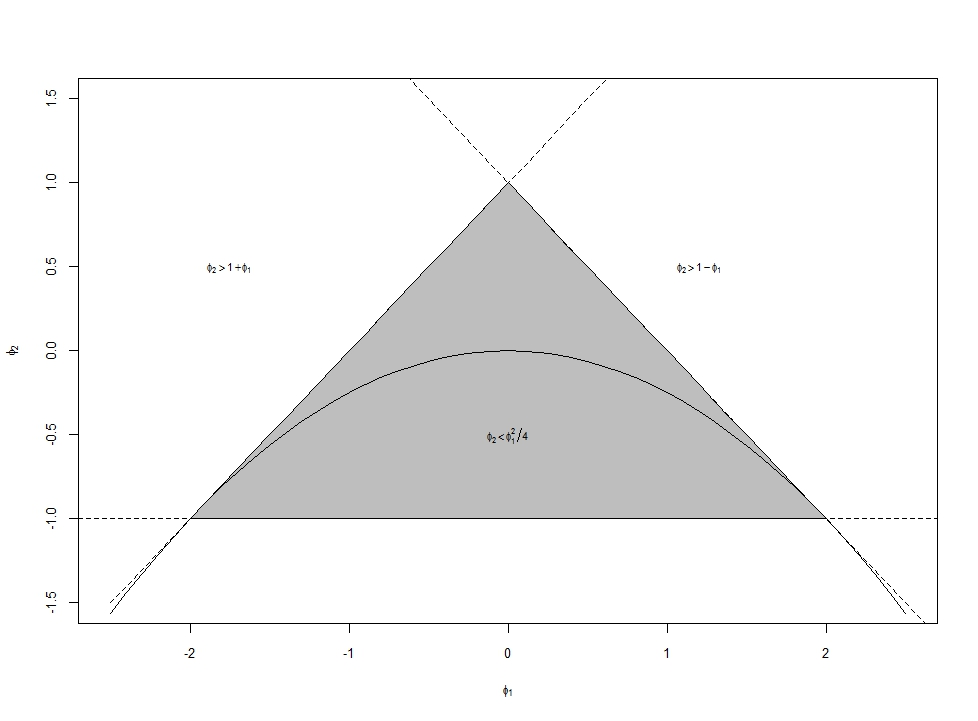
\includegraphics[width=0.8\textwidth]{figures/AR(2).jpg}
    %     \caption{Stationarity Region for AR(2) processes}
    %     \label{fig:AR2}
    % \end{figure}

    \begin{theorem}[AR(2) Stationarity]\label{thm:AR2stationarity}
        \

        If $\mathbb{E}\vert e_t \vert < \infty,$ and $\vert \lambda_j \vert < 1$ for $\lambda_j$ defined in \eqref{eq:lambdadef}, then the AR(2) process is stationary,
        or equivalenetly, the following inequalities hold:
        \begin{gather}
            \phi_1 + \phi_2 < 1 \\
            \phi_2 - \phi_1 < 1 \\
            \phi_2 > -1
        \end{gather}
        then, the AR(2) process \eqref{eq:AR2} is absolutely convergent, strictly stationary, and ergodic.
    \end{theorem}
\end{eg}

\subsection{Moving Average Models (MA\texorpdfstring{$(q)$}{(q)})}\label{sec:MA}

As an alternative to the autoregressive representation in which the $y_t$ on the left-hand
side of the equation are assumed to be combined linearly, the moving average model
of order q, abbreviated as MA$(q)$, assumes the white noise $u_t$ on the right-hand side
of the defining equation are combined linearly to form the observed data.

If $\phi(B) \equiv 1$ in ARMA$(p,q)$ \ref{eq:ARMApq}, then we have the \textbf{moving average} model of order $q$ (MA$(q)$):
\begin{definition}[MA$(q)$ Process]\label{def:MAq}
    \
    
    The process $\{ y_t, t=0, \pm1, \pm2, \cdots\}$ is said to be an MA$(q)$ process if $y_t$ is stationary and for every $t$,
    \begin{gather}\label{eq:MAq}
        y_t = \alpha + u_t + \theta_1 u_{t-1} + \cdots + \theta_q u_{t-q}
    \end{gather}
    where $u_t \sim WN(0,\sigma^2)$, $\alpha = \mu$, $\mathbb{E}[y_t] = \mu$, and $\theta_q \neq 0.$
    This can be written symbolically in the more compact form:
    \begin{gather*}
        y_t = \alpha + \theta(B) u_t, t = 0, \pm1, \pm2, \cdots
    \end{gather*}
    where $\theta (B) = 1 + \theta_1 B + \cdots + \theta_q B^q$.
\end{definition}
It's quite easy to see that the `\textbf{linear process}' we defined in \ref{thm:wolddecomp} is $MA(\infty)$ and the white noise process is $MA(0)$.
We can obtain $\mathbb{E}[y_t] = \alpha$ and:
\begin{align*}
    \gamma(h) &= \Cov[y_{t+h}, y_t] = \Cov[u_{t+h} + \theta_1 u_{t+h-1} + \cdots + \theta_q u_{t+h-q}, u_t + \theta_1 u_{t-1} + \cdots + \theta_q u_{t-q}]\\
    &= \mathbb{E}\left[(u_t + \theta_1 u_{t-1} + \cdots)(u_{t+h} + \theta_1 u_{t+h-1} + \cdots)\right]\\
    &= \begin{dcases}
        \sigma^2 \sum_{j=0}^{q-\vert h\vert}\theta_j \theta_{j + \vert h \vert} , & \vert h \vert < q;\\
        0, & \vert h \vert > q.
    \end{dcases}
\end{align*}


\begin{eg}[MA(1) Process]\label{eg:MA1}
    \
    
    The MA(1) process is given by
    \begin{gather}\label{eq:MA1}
        y_t = \alpha + u_t + \theta u_{t-1}, \quad u_t \sim WN(0, \sigma^2).
    \end{gather}
    The model is called a ``moving average'' because $y_t$ is a weighted average of the shocks $u_t$ and $u_{t-1}$.
    We can obtain that $\mathbb{E}[y_t] = \alpha$ and:
    \begin{align*}
        \gamma(h) &= \Cov[y_{t+h}, y_t] = \Cov[u_{t+h} + \theta u_{t+h-1}, u_t + \theta u_{t-1}]\\
        &= \mathbb{E}\left[(u_t + \theta u_{t-1})(u_{t+h} + \theta u_{t+h-1})\right]\\
        &= \begin{dcases}
            (1+\theta^2) \sigma^2, &\text{ if } h = 0;\\
            \theta \sigma^2, &\text{ if } h = \pm1;\\
            0, &\text{ otherwise} .
        \end{dcases}
    \end{align*}
    Thus $y_s$ and $y_t$ are uncorrelated whenever $s$ and $t$ are two or more times instants apart.
    Therefore, the MA(1) process is weak stationary regardless of the value of $\theta$.
    We speak of \textit{short range dependence} and say that the time series has \textit{short memory}.
\end{eg}


% \subsection{Trend and Seasonality}\label{sec:trendseasonality}
% In reality, raw data is seldom stationary. It often displays a trend as well as some regular, fluctuating
% pattern, referred to as ``seasonality''.
% One possible treatment of data is to assume that the data set is a realization of the stochastic
% process $X_t$ can be split into:
% \begin{gather*}
%     X_t = m_t + s_t + y_t
% \end{gather*}
% where $m: \mathbb{Z} \to \mathbb{R}$ is a slowly changing function called the \textit{trend component};
% $s: \mathbb{Z} \to \mathbb{R}$ is a function with known period $d$ called the \textit{seasonal component}, i.e. $s_{t+d} = s_t$ and $\sum_{j=0}^{d} s_j = 0$;
% and $y_t$ is a stationary process with mean zero and finite variance.

% \begin{note}
%     \

%     Once the trend and seasonality are subtracted, we would be left with yt, which is typically WS
% and can be modeled as an ARMA process. (Alternatively, if it displays some instability that
% (potentially) prevents it from being WS, we can model its dynamics using more advanced
% models that display, for example, conditional heteroskedasticity, stochastic volatility or time-
% varying parameters.)
% \end{note}

